%%
%% VERSION HISTORY
%%    22 May 2006 - John Papandriopoulos - Original version
%%    12 Jul 2007 - John Papandriopoulos - Converted into template
%%

\chapter{Tools and resources}
	\label{chapter:empire-strikes-back}%
	%

% preferred location for figures in this chapter
\setfigurepath{figures/chapter-3}

%=========================================================================

%=========================================================================
\section{Employed NLP methods}
\subsection*{Tokenization}
\textit{Tokenization} is usually a crucial step appearing in early stage of the NLP workflow to facilitate processing with more complex analytical techniques. Tokenization is the task of divide a character sequence into defined document units referred as tokens. A token is defined as "an instance of a sequence of characters in some particular document that are grouped together as a useful semantic unit for processing" \cite{Manning:2008:IIR:1394399}. In theory, tokens can take form of any textual elements of chosen granularity such as punctuation or fomulae but in practice, tokens are usually words.\\

\begin{figure}
\centering
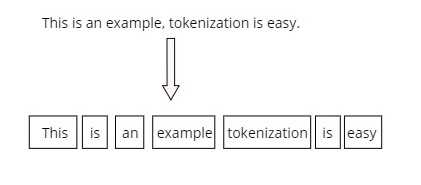
\includegraphics[width=\textwidth, clip=true, height = 5.5cm]{img/tokenization_example}
\caption[Tokenization example]{ Example of tokenization. Tokenizer splits a sentence into words.
} 
\label{fig:token_ex1}
\end{figure}

As shown in Figure~\ref{fig:token_ex1}, tokenization have dropped punctuation of the sentence and each word is getting full meaning. However, tokenization phase may encounters difficult choice in a broader context. For example, take a look at the sentence "\textit{Tokenization isn't easy}". Two words \framebox{Tokenization} and \framebox{easy} are pretty straightforward since they are splitted by whitespace. In contrast, \textit{isn't} can be tokenized by different rules: \framebox{isn't}, \framebox{isnt}, \framebox{is} \framebox{n't}, \framebox{isn} \framebox{t}. Furthermore, each language and topic contain jargon and words refer to specific entities but are not in standard dictionary. For instance, AK-47 is name of a semi-automatic rifle, programming language C\# and so on. Computer era brings new types of technology terminology, which appear frequently on online document, such as website addresses (https://www.google.com/), email adresses (johndoe@gmail.com), decimal IP addresses (123.172.2.1). These character sequences should be recognize as one entity but in some cases, it would cause unnecessary index to be included in the extracted dictionary. In the experiment of this thesis, NLTK Tokenizer package, which is improved TreebankWordTokenizer \footnote{http://www.nltk.org/api/nltk.tokenize.html\#nltk.tokenize.treebank.TreebankWordTokenizer} along with PunktSentenceTokenizer \footnote{http://www.nltk.org/api/nltk.tokenize.html\#nltk.tokenize.punkt.PunktSentenceTokenizer} for the specified language, was used.

\subsection*{Stop words removal}
\textit{Stop words} are words that contribute very little in term of semantic, thus being considered low value in IR systems. These words usually appear with high frequency in collection. To remove stop words, high use words must be manually assessed for semantic content. If a word is identify as a stop word, it is added to a list called \textit{stop list}. The length of a stop list varies between less than twenty (15-18 terms) to a few hundred words (200-300 terms). Depeding on purpose and scale of a system, a stop list can be very general or specifically relate to a topic.\\
Using a stop list can potentially reduce query time due to smaller index of a system. However, web search engines in practice do not use stop lists partially because of immense server clusters behind them generating enormous computing power. \\
Common words belong to world classes article, conjunction, preposition and frequent words like \textit{now} or \textit{very} are included in stop lists. General-purpose stop lists are available online and can be easily incorporated into IR systems. Sometimes removing stop words can be detrimental as vital information may be missed after going through stop list filter (e.g. \textit{"To be or not to be"} is a well known verse that may get taken out of indexed vocabulary) so utilization of these lists must be carefully examined. 
 In the experiment of this thesis, Stopwords corpus of NLTK was used. It is a corpus containing 2400 stopwords for 11 languages. Stop list for English contain 153 words.